\chapter{Approach}	\label{chapter:approach}

\section{Algorithmic Design}
\label{chapter:approach:algorithmic_design}

The algorithmic structure of MABDI can be seen in system diagram shown in Fig.
\ref{fig:system}. Table \ref{tab:var} gives a description of the main variables.

\begin{figure}[h]%[thpb]
\centering
  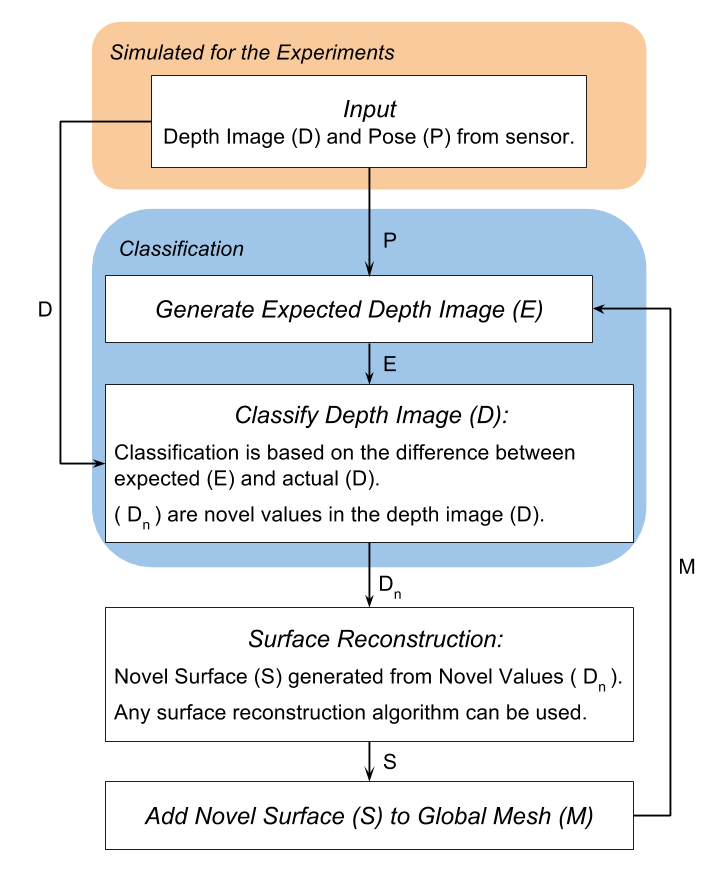
\includegraphics[width=.75\textwidth]{figures/diagram_system.png}
  \caption{MABDI system diagram}
  \label{fig:system}
\end{figure}

\begin{table}[h]
  \caption{Basic description of the main variables}
  \label{tab:var}
  \begin{center}
    \begin{tabular}{|c|l|}
    \hline
    {\bf Variable Name} & \multicolumn{1}{|c|}{{\bf Description}} \\
    \hline
    \rowcolor{LightGray} $D$ & Depth image from RGB-D sensor \\
    $P$ & Pose of the sensor \\
    \rowcolor{LightGray} $D_n$ & Parts of $D$ that are \emph{novel} \\
    $S$ & Novel surface generated from $D_n$ \\
    \rowcolor{LightGray} $M$ & Global mesh \\
    \hline
    \end{tabular}
  \end{center}
\end{table}


The system diagram is very similar to Fig. \ref{fig:pipeline} with the exception
of the Classification component, shown in blue. This Classification component is
MABDI's contribution to the state-of-art in mesh based mapping algorithms, and
is what gives MABDI the ability to make decisions about the incoming data. The
Classification component consists of two elements:
\begin{enumerate}
    \item \textit{Generate Expected Depth Image $E$} - Here we take the global
    mesh $M$, render it using computer graphics, and use the depth buffer of the
    render window to create a depth image $E$ of what we expect to see from our
    sensor. This method requires the current pose $P$ of the actual sensor
    (simulated for our experiments).
    \item \textit{Classify Depth Image $D$} - Here we classify the actual depth
    image $D$ (simulated for our experiments) by first taking the absolute
    difference between $E$ and $D$ and thresholding. If the differences are
    small, those points are thrown away and if the differences are large, those
    points are kept as $D_n$. The idea behind this is, if the difference is
    large, the measurements are coming from a part of the environment that has
    not been seen before, i.e. novel. The implication of this assumption is that
    this version of MABDI cannot handle object removal. It is worth noting
    that MABDI can be extended to handle object removal by using the sign of the
    difference between $E$ and $D$ instead of the absolute value.
\end{enumerate}

% Simulated for the Experiments
The system diagram in Fig. \ref{fig:system} also shows the Input and the Surface
Reconstruction components. The Input component has been simulated for our
experiments. More details of this simulation will be covered in Section
\ref{chapter:experimental_setup}. The Surface Reconstruction component of the
MABDI algorithm can be implemented with any viable surface reconstruction
method. Our implementation utilizes the structural information contained within
the depth image. We will discuss this in more detail in the next section.

\section{Implementation}

\subsection{Surface Reconstruction}

A depth image is not simply a set of unorganized points, but has inherent
structural information as well. This characteristic of the depth image allows us
to define a topology on the 2 dimensional depth image that is preserved when
projected to real-world coordinates. Our surface reconstruction method defines a
topology that is visualized in Fig. \ref{fig:srm}. Here elements of the mesh
are shown in light blue and novel points $D_n$ are shown as blue dots. The red
dot signifies a point that is not from the set $D_n$. Our implementation removes
all mesh elements touching such points, as seen in the figure.

\begin{figure}[h]%[thpb]
\centering
  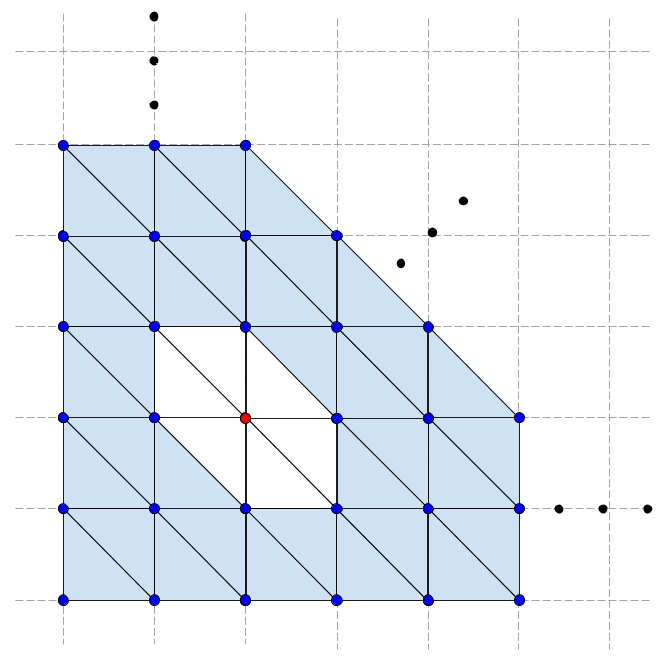
\includegraphics[width=.6\textwidth]
    {figures/diagram_surface_reconstruction.png}
  \caption{Surface reconstruction method}
  \label{fig:srm}
\end{figure}

Our surface reconstruction methods was chosen for its ability to be implemented
simply and run quickly. One consequence of our method is that the resulting
surface $S$ can have a large amount of elements. For example, if all points from
$D$ are classified as novel (this happens on the first frame), $S$ can contain
over $600,000$ elements. This assumes $D$ has no invalid points, e.g., out of
the sensor's range. Many surface reconstruction methods have been developed to
create a surface more intelligently, as discussed in Section
\ref{chapter:related_works}. For example, the advancing front method developed
by Marton et al. \cite{Marton2009} is capable of creating surfaces with fewer
elements by utilizing robust resampling methods. One great thing about the MABDI
algorithm is that the method developed by Marton et al. can be used in place of
our surface reconstruction method. Also, due to our implementation's modular
software design, the entire code base would not need to be changed in order to
accomplish this. We will discuss the software design in the next section.

\subsection{Software Design}

From a software perspective, the major difficulty of implementing the MABDI
algorithm was found to be creating both the simulated depth image $D$ and the
expected depth image $E$. In addition, managing the complexity of the data
pipeline needed to run the algorithm and the simulation of the sensor proved to
be difficult. Thankfully, Kitware, who is a leading edge developer of
open-source software, created the Visualization Toolkit (VTK)
\cite{schroeder2004visualization, sitevtk}. At the time of this writing the VTK
Github repository has over 60,000 commits and is contributed to by supporters
such as Sandia National Labs \cite{sitesandia}.

VTK is aptly designed for the implementation of MABDI for many reasons. Perhaps
the most important is the concept of a vtkAlgorithm (often called a Filter).
This allows a programmer to create a custom and modular processing pipeline by
defining classes that inherit vtkAlgorithm and then defining the connections
between these classes. For example, you could have a pipeline that reads an
image from a source (component 1), performs edge detection (component 2), and
then renders the image (component 3). Using this concept, the individual
elements of MABDI can be succinctly defined in individual classes. With that in
mind, we can see in Fig. \ref{fig:software} the layout used in my implementation
of MABDI. Note, vtkImageData and vtkPolyData are VTK types used to represent an
image and mesh respectively:

\begin{itemize}
    \item  \textit{Source} - Classes with the prefix Source define the
    environment that is used for the simulation and provide a mesh in the form
    of a vtkPolyData.
    \item \textit{FilterDepthImage} - Render the incoming vtkPolyData in a
    window and output the depth buffer from the window as a vtkImageData. The
    output additionally has pose information of the sensor.
    \item \textit{FilterClassifier} - Implements the true innovation of MABDI,
    takes the difference between the two incoming depth images (vtkImageData)
    and outputs a new depth image where the data that is not novel is marked to
    be thrown away.
    \item \textit{FilterDepthImageToSurface} - Performs surface reconstruction
    on the novel points. In this simple implementation the topology of the mesh
    is defined in the image coordinates and can be thought of as a checkerboard
    pattern with two triangles in every square. The data is then projected to
    real-world coordinates. The topology and the real-world coordinates are
    combined to define a surface and output as a vtkPolyData.
    \item \textit{FilterWorldMesh} - Here we simply append the incoming novel
    surface to a growing global mesh that is also output as a vtkPolyData.
\end{itemize}

\begin{figure}[h]%[thpb]
\centering
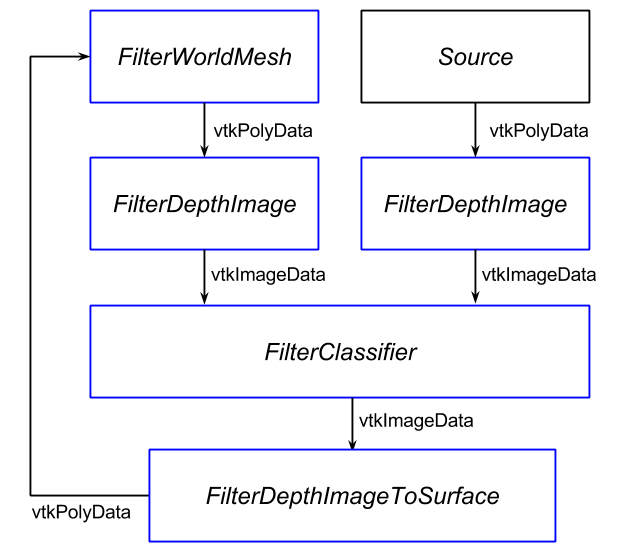
\includegraphics[width=.75\textwidth]{figures/diagram_software.png}
\caption{MABDI software diagram}
\label{fig:software}
\end{figure}

MABDI is implemented in Python and uses VTK. Our implementation is distributed
under the BSD license and is available on Github at the address below:

$$
https://github.com/lucasplus/MABDI
$$

At the time of this writing, it consists of over 1,400 lines. The code that
implements the MABDI algorithm itself is around 750 lines.
